\documentclass[12pt, a4paper]{article}

\usepackage[utf8]{inputenc}
\usepackage[T2A]{fontenc}
\usepackage[russian]{babel}
\usepackage{amsmath, amsthm, amssymb}
\usepackage[hidelinks]{hyperref}
\usepackage{geometry}
\usepackage{graphicx}
\usepackage{tikz}
\usetikzlibrary{positioning}
\definecolor{PaleGreen}{rgb}{0.59375, 0.98046875, 0.59375}
\definecolor{LimeGreen}{rgb}{0.2, 0.8, 0.2}
\definecolor{MediumBlue}{rgb}{0, 0, 0.8}

\geometry{top=2.5cm, bottom=2.5cm, left=2.5cm, right=2.5cm}

\theoremstyle{definition}
\newtheorem*{definition}{Определение}
\theoremstyle{plain}
\newtheorem*{theorem}{Теорема}
\newtheorem*{statement}{Утверждение}
\newtheorem*{lemma}{Лемма}
\newtheorem*{corollary}{Следствие}
\theoremstyle{remark}
\newtheorem*{remark}{Замечание}

\title{\textbf{Декартовы деревья и range-деревья}}
\author{}
\date{}

\begin{document}

\maketitle
\tableofcontents
\newpage

%%%%%%%%%%%%%%%%%%%%%%%%%%%%%%%%%%%%%%%%%%
\section{Декартово дерево}
%%%%%%%%%%%%%%%%%%%%%%%%%%%%%%%%%%%%%%%%%%

\subsection{Мотивация и основная идея}

Обычное BST (двоичное дерево поиска) без балансировки может выродиться в список, из-за чего операции поиска/вставки/удаления и т.д. будут работать долго. Хотим придумать структуру с гарантированной средней глубиной $O(\log n)$.

\begin{definition}
\textit{Декартово дерево (ДД)}~--- бинарное дерево, в узлах которого хранятся
пары $(x, y)$, являющееся одновременно BST по $x$ и кучей
по $y$. Координата $x$ называется \textit{ключом}, а координата $y$ ~--- приоритетом. Для удобства в дальнейшем давайте считать, что куча по $y$ - это max-куча. 
\end{definition}

\begin{statement}
При различных ключах и приоритетах декартово дерево \textbf{единственно}.
\end{statement}

\begin{proof}
Корнем точно будет вершина с максимальным $y$, оставшиеся вершины разбиваем на группы с ключом меньше ключа корня и больше ключа корня, для них рекурсивно повторяем рассуждение.
\end{proof}
\subsection{Операции split и merge}

Все операции сводятся к двум базовым операциям (\textbf{split} и \textbf{merge}). Каждая из этих операций будет делать единственный рекурсивный вызов от дерева глубины на $\geq 1$ меньше, а значит они будут работать за $O(h)$, где $h$ ~--- глубина.

\medskip
\noindent\textbf{split}$(T, k) \to \langle L, R \rangle$~--- разрезать ДД $T$ по ключу $k$, то есть разбить на два ДД: в $L$ должны попасть вершины с ключами $< k$, в $R$~--- остальные.

Работает \textbf{split} так: если $k > x_{\mathrm{root}}$~--- рекурсия уходит в правое поддерево (см. рис. 1), иначе~--- в левое.

\smallskip
\noindent\textbf{merge}$(L, R) \to T$~--- объединить два ДД при условии, что ключи $L <$ ключи $R$. 

Устройство \textbf{merge}: пусть приоритет корня $L$ больше приоритета корня $R$ (другой случай аналогичен), его возьмем корнем. Тогда в качестве итогового ДД подойдет такое дерево: к уже выбранному корню слева прикрепляем левое поддерево $L$, а справа прикрепляем результат \textbf{merge} $R$ и правого поддерева $L$ (см. рис. 2). 

\begin{figure}[h]
    \centering
    \begin{minipage}[t]{0.45\textwidth}
        \centering
        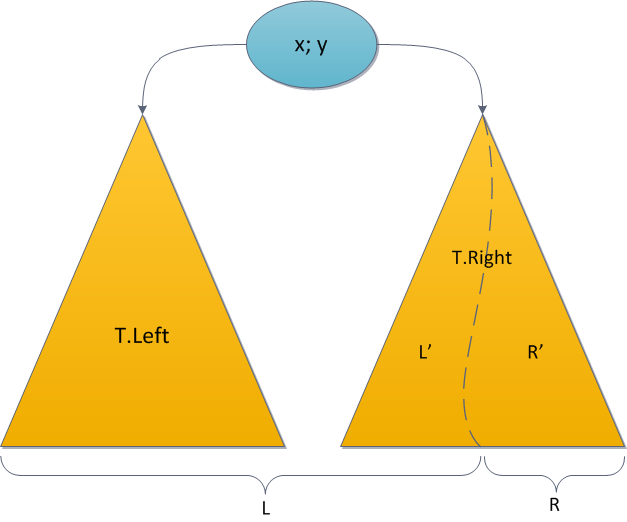
\includegraphics[width=\textwidth]{treap-range-img/split.png}
        \caption{Операция \textbf{split}}
        \label{split}
    \end{minipage}
    \hfill 
    \begin{minipage}[t]{0.5\textwidth}
        \centering
        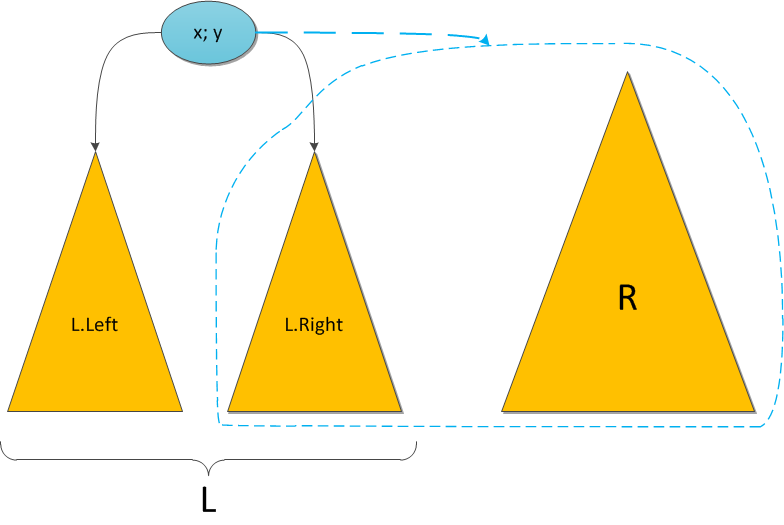
\includegraphics[width=\textwidth]{treap-range-img/merge.png}
        \caption{Операция \textbf{merge}}
        \label{merge}
    \end{minipage}
\end{figure}


\noindentИз полученных операций можно легко реализовать интерфейс \textbf{set}:

\medskip
\noindent\textbf{insert}$(T, v)$ ~--- добавить вершину $v$ (ключ и приоритет):

Делаем split по $v.x$ (получим $L$ и $R$), после делаем слияние $L$ и $v$ (из одной вершины всегда можно построить дерево), результат нужно слить с $R$. 

\noindent\textbf{remove}$(T, x)$ ~--- удалить вершину с ключом $x$:

Делаем split по $x$ (получим $L$ и $R$), удаляем у $R$ самую левую вершину, если её ключ равен $x$ (получим $R'$), сливаем $L$ и $R'$.

\subsection{Построение за $O(n)$}
Данный алгоритм работает только в случае, когда точки $(x_1, y_1), ..., (x_n, y_n)$ уже отсортированы по $x$ (по возрастанию). В противном случае время работы $O(n\log n)$ из-за сортировки.

Строим итеративно слева направо, при вставке очередного $(x_k, y_k)$ идем по самой правой ветви дерева снизу вверх и находим первую вершину $v$ с приоритетом больше $y_{k}$. Если такой нет, текущее дерево делаем левым поддеревом $(x_k, y_k)$; иначе на этой итерации изменим дерево так: вершине $(x_k, y_k)$ слева подвесим правое поддерево $v$, а справа - ничего; вершине $v$ вместо правого поддерева подвесим вершину $(x_k, y_k)$. 

\begin{figure}[h]
\centering
\begin{tikzpicture}[
  nd/.style  = {circle, draw=black!65, fill=white,
                minimum size=8.5mm, inner sep=0pt, line width=0.8pt},
  vnd/.style = {circle, draw=orange!80!black, fill=orange!20,
                minimum size=8.5mm, inner sep=0pt, line width=1.1pt},
  und/.style = {circle, draw=LimeGreen!65!black, fill=PaleGreen,
                minimum size=8.5mm, inner sep=0pt, line width=0.8pt},
  nnd/.style = {circle, draw=MediumBlue, fill=MediumBlue!10,
                minimum size=8.5mm, inner sep=0pt, line width=1.1pt},
  sp/.style  = {draw=black!55, line width=0.8pt},
  >=stealth,
]

\begin{scope}
  \node[nd]  (A1) at (0,  0.0) {};
  \node[nd]  (A2) at (0, -1.6) {};
  \node[vnd] (Av) at (0, -3.8) {};
  \node[und] (Au) at (0, -5.3) {};
  \node[nd]  (Al) at (0, -7.3) {};

  \draw[sp] (A1)--(A2);
  \draw[sp] (A2)--(Av);
  \node[fill=white, inner sep=2pt] at (0,-2.8) {$\vdots$};
  \draw[sp] (Av)--(Au);
  \draw[sp] (Au)--(Al);
  \node[fill=white, inner sep=2pt] at (0,-6.4) {$\vdots$};

  \foreach \name/\ny in {A1/0.0, A2/-1.6, Av/-3.8, Au/-5.3, Al/-7.3}{
    \draw[teal!50!black, dashed, line width=0.55pt]
      (\name.west) -- (-1.05, \ny-0.50);
    \fill[teal!15, draw=teal!58!black, line width=0.6pt]
      (-1.47,\ny-1.15) -- (-0.63,\ny-1.15) -- (-1.05,\ny-0.50) -- cycle;
  }

  \draw[->, gray!55, line width=0.9pt]
    (Al.east) to[bend right=40] (Av.east);

  \node[nnd] (Anew) at (2.5,-3.8) {};
\end{scope}

\draw[->, line width=1.6pt, gray!40] (3.5,-4.5) -- (4.8,-4.5);

\begin{scope}[xshift=8.2cm]
  \node[nd]  (B1)   at (0,  0.0) {};
  \node[nd]  (B2)   at (0, -1.6) {};
  \node[vnd] (Bv)   at (0, -3.8) {};
  \node[nnd] (Bnew) at (0, -5.3) {};

  \draw[sp] (B1)--(B2);
  \draw[sp] (B2)--(Bv);
  \node[fill=white, inner sep=2pt] at (0,-2.8) {$\vdots$};
  \draw[sp] (Bv)--(Bnew);

  \foreach \name/\ny in {B1/0.0, B2/-1.6, Bv/-3.8}{
    \draw[teal!50!black, dashed, line width=0.55pt]
      (\name.west) -- (-1.05, \ny-0.50);
    \fill[teal!15, draw=teal!58!black, line width=0.6pt]
      (-1.47,\ny-1.15) -- (-0.63,\ny-1.15) -- (-1.05,\ny-0.50) -- cycle;
  }

  \draw[LimeGreen!55!black, dashed, line width=0.65pt]
    (Bnew.west) -- (-1.05,-5.75);
  \fill[PaleGreen!75, draw=LimeGreen!55!black, line width=0.8pt]
    (-1.57,-6.58) -- (-0.53,-6.58) -- (-1.05,-5.75) -- cycle;
\end{scope}

\node[nd,  minimum size=5.5mm] at (0.5,-10.3) {};
\node[font=\scriptsize, anchor=west] at (1.05,-10.3)
  {узел правой ветви};

\node[vnd, minimum size=5.5mm] at (0.5,-11.0) {};
\node[font=\scriptsize, anchor=west] at (1.05,-11.0)
  {первая вершина $v$ с $y_v > y_k$};

\node[und, minimum size=5.5mm] at (0.5,-11.7) {};
\node[font=\scriptsize, anchor=west] at (1.05,-11.7)
  {последняя с $y < y_k$, корень правого поддерева $v$};

\node[nnd, minimum size=5.5mm] at (0.5,-12.4) {};
\node[font=\scriptsize, anchor=west] at (1.05,-12.4)
  {новый узел $(x_k,\,y_k)$};

\fill[teal!15, draw=teal!58!black, line width=0.6pt]
  (5.2,-10.10) -- (5.8,-10.10) -- (5.5,-9.78) -- cycle;
\node[font=\scriptsize, anchor=west] at (5.95,-9.95)
  {левое поддерево вершины};

\fill[PaleGreen!75, draw=LimeGreen!55!black, line width=0.8pt]
  (5.2,-10.80) -- (5.8,-10.80) -- (5.5,-10.48) -- cycle;
\node[font=\scriptsize, anchor=west] at (5.95,-10.65)
  {правое\ поддерево $v$ до добавления $(x_k, y_k)$};

\end{tikzpicture}
\caption{
  Шаг алгоритма построения ДД за $O(n)$: вставка узла $(x_k,\,y_k)$.
  Серая стрелка показывает подъём по правой ветви снизу вверх
  до первой вершины~$v$ с~$y_v>y_k$.}
\end{figure}

При таком алгоритме все вершины посещены $\leq 2$ раз (при добавлении 1 раз, при втором посещении мы ее отправляем в левое поддерево, а алгоритм всегда шагает по самой правой ветке), время работы: $O(n)$.

\subsection{Случайные приоритеты и высота}

\begin{theorem}
В декартовом дереве из $n$ узлов со случайными одинаково распределенными приоритетами верно: $\mathbb{E}[d(x_k)] = O(\log n)$, где $d(x_k)$ - глубина $k$-й вершины.
\end{theorem}

\begin{proof}
Для удобства $x_1 < x_2 < ... < x_n$. 
\begin{enumerate}
  \item Индикатор $A_{i,k} := 1 \Leftrightarrow x_i$~--- предок $x_k$.
        Тогда $d(x_k) = \sum_i A_{i,k}$, и по линейности матожидания
        $\mathbb{E}[d(x_k)] = \sum_i \Pr[A_{i,k} = 1]$.

  \item \textbf{Лемма.} $x_i$~--- предок $x_k$ $\Leftrightarrow$ $x_i$ имеет
        наибольший приоритет в $X_{i,k} = \{x_{\min(i,k)},\ldots,x_{\max(i,k)}\}$.

        \textit{Доказательство (индукция по размеру поддерева):}
        если корень~--- $x_i$, то он предок и имеет максимальный приоритет;
        если корень~--- $x_k$, то $x_i$ не предок и не максимален в $X_{i,k}$;
        если корень~--- $x_m$ между $i$ и $k$, то $x_m\in X_{i,k}$, и $x_i$
        не предок; иначе~--- рекурсия на меньшее поддерево.

  \item Из равномерности: $\mathbb{P}[A_{i,k}=1] = \dfrac{1}{|k-i|+1}$.

  \item Итого:
        $\mathbb{E}[d(x_k)] = \displaystyle\sum_{i\neq k}\frac{1}{|k-i|+1}
        \leq \ln k + 1 + \ln(n-k) + 1 = O(\log n)$.\qedhere
\end{enumerate}
\end{proof}

\begin{corollary}
Среднее время указанных операций над ДД ~--- $O(\log n)$.
\end{corollary}

\subsection{Декартово дерево по неявному ключу}

\textbf{Мотивация:} Хотим эффективно реализовать динамический массив с вставкой/удалением в произвольную позицию и операциями на отрезке.

\textbf{Идея:} Не будем хранить ключ $x$ явно, но будем подразумевать, что в вершинах ДД он есть автоматически. Для удобства можно считать, что в дереве из $n$ вершин ключами будут числа $0, 1, ..., n - 1$. Заметим, что их расположение в вершинах дерева однозначно восстанавливается по структуре дерева. Значит можно считать наше дерево массивом в том смысле, что на месте $i$ будет стоять элемент, у которого есть неявный ключ $i$.

\textbf{Операции:}

\noindent\textbf{merge}$(L, R)$ - дописать в конец массива $L$ массив $R$. Заметим, что реализация \textbf{merge} для обычного ДД не пользовалась ключами, а лишь предполагала, что ключи в $L <$ ключей $R$. Тогда эта реализация подойдет. 

Для реализации операции \textbf{split} нужно хранить дополнительную информацию: в каждой вершине хранится $C$~--- размер поддерева. 

\noindent\textbf{split}$(T, k)$ теперь отрезает ровно $k$ вершин от ДД $T$: если $l = |T.\mathit{left}| \geq k$~--- рекурсия в левом поддереве с параметром $k$;
иначе~--- в правом с параметром $k - l - 1$. После изменений детей как в обычном \textbf{split} обновляем размеры поддеревьев там, где они поменялись. Сложность времени работы не изменилась.

\textbf{Применения:} логарифмическое время на все следующее: вставка на фиксированную позицию, удаление, перестановка подотрезка, массовые операции на отрезке (аналогично ДО).

%%%%%%%%%%%%%%%%%%%%%%%%%%%%%%%%%%%%%%%%%%
\section{Range-деревья}
%%%%%%%%%%%%%%%%%%%%%%%%%%%%%%%%%%%%%%%%%%

\subsection{Постановка задачи}

Дано множество из $n$ точек в $\mathbb{R}^d$; хотим отвечать на
запросы вида <<найти все точки в прямоугольном гиперпараллелепипеде $[x_1:x_1'] \times [x_2: x_2'] \times \ldots \times [x_d: x_d']$>>. Рассмотрим \textbf{range-деревья}, которые имеют ряд преимуществ в сравнении с другими известными структурами данных (например kd-tree). Итоговая сложность будет такая:

\begin{center}
\begin{tabular}{l|c|c|c}
Структура & Построение & Память & Запрос \\
\hline
kd-tree & $O(n\log n)$ & $O(n)$ & $O(n^{1-\frac{1}{d}}+k)$ \\
\hline
Range-tree & $O(n\log^{d-1} n)$ & $O(n\log^{d-1} n)$ & $O(\log^d n+k)$ \\
Layered range-tree & $O(n\log^{d-1} n)$ & $O(n\log^{d-1} n)$ & $O(\log^{d-1} n+k)$ \\
\end{tabular}
\end{center}

Здесь $k$~--- число найденных точек в гиперпараллепипеде для данного запроса.

\subsection{Одномерный случай}

Прежде чем перейти к многомерным range-деревьям, разберём одномерный случай: дано множество $P = \{p_1, \ldots, p_n\}$ вещественных чисел, запросы вида $[x : x']$.

\textbf{Структура данных.} Храним $P$ в листьях сбалансированного BST $T$. Внутренние вершины хранят значение для разделения, листья~--- сами точки.


\begin{definition}
    \textit{Каноническое подмножество} вершины дерева ~--- множество листьев её поддерева. Для вершины $\nu$ ее каноническое подмножество будем обозначать $P(\nu)$.
\end{definition}

\textbf{Алгоритм запроса} \textsc{1DRangeQuery}$(T, [x:x'])$:
\begin{enumerate}
    \item Делаем два поиска в BST для $x$ и $x'$, находим $\nu_{\mathrm{split}}$~--- вершину, где пути поиска $x$ и $x'$ расходятся.
    \item Идём по пути к $x$: на каждом шаге влево возвращаем листья правого поддерева.
    \item Идём по пути к $x'$: на каждом шаге вправо возвращаем листья левого поддерева.
    \item Проверяем листья путей поиска, в которых пути заканчиваются ($\mu$ и $\mu'$).
\end{enumerate}

\begin{figure}[h!]
    \centering
    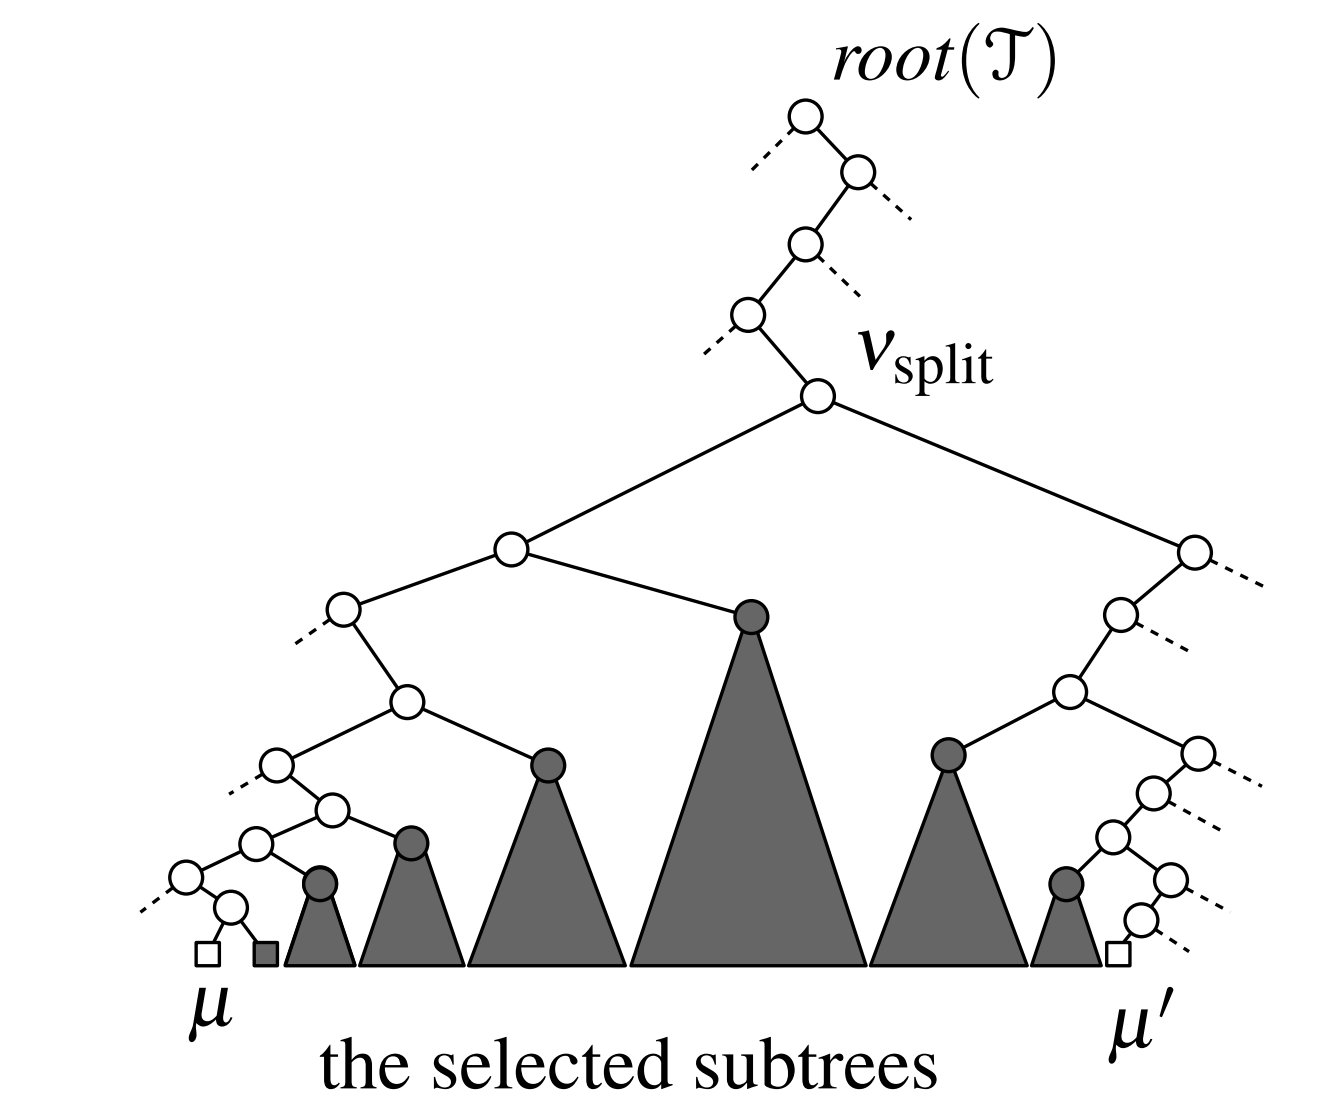
\includegraphics[width=0.4\textwidth]{treap-range-img/bst.png}
    \caption{\textsc{1DRangeQuery}}
    \label{bst}
\end{figure}

\begin{theorem}
Множество $P$ из $n$ точек в $\mathbb{R}^1$ можно хранить в сбалансированном BST, использующем $O(n)$ памяти и строящемся за $O(n\log n)$ так, что ответ на запрос $[x:x']$ тратит $O(\log n + k)$ времени, где $k$~--- число найденных точек запроса.
\end{theorem}

\begin{proof}
Корректность очевидна, время работы следует из того, что поиск в BST тратит $O(\log n)$, а возврат $k$ найденных точек из листьев займет $O(k)$, так как в поддереве листья занимают $\geq \frac{1}{2}$ всех вершин поддерева.
\end{proof}

\begin{remark}
    \textbf{Важно отметить}, что возвращений левых/правых поддеревьев будет $O(\log n)$ (в силу сбалансированности дерева), то есть любой отрезок представляется в виде дизъюнктного объединения канонических подмножеств $O(\log n)$ вершин, при том эти вершины мы находим за $O(\log n)$.
\end{remark}


\subsection{Двумерный случай}

\textbf{Главная идея:} превратить двумерный запрос $[x:x'] \times [y:y']$ в два одномерных (с которыми мы уже умеем работать!).

\begin{definition}
\textit{Range-дерево} для набора $P$ из $n$ точек плоскости~--- двухуровневая структура:
\begin{itemize}
    \item \textit{Главное дерево} $T$~--- сбалансированный BST по $x$-координатам;
    \item Каждая вершина $\nu \in T$ хранит указатель на \textit{ассоциированную структуру} $T_{\mathrm{assoc}}(\nu)$~--- сбалансированное BST по $y$-координатам точек из канонического подмножества ~--- $P(\nu)$.
\end{itemize}
\end{definition}

\begin{figure}[h!]
    \centering
    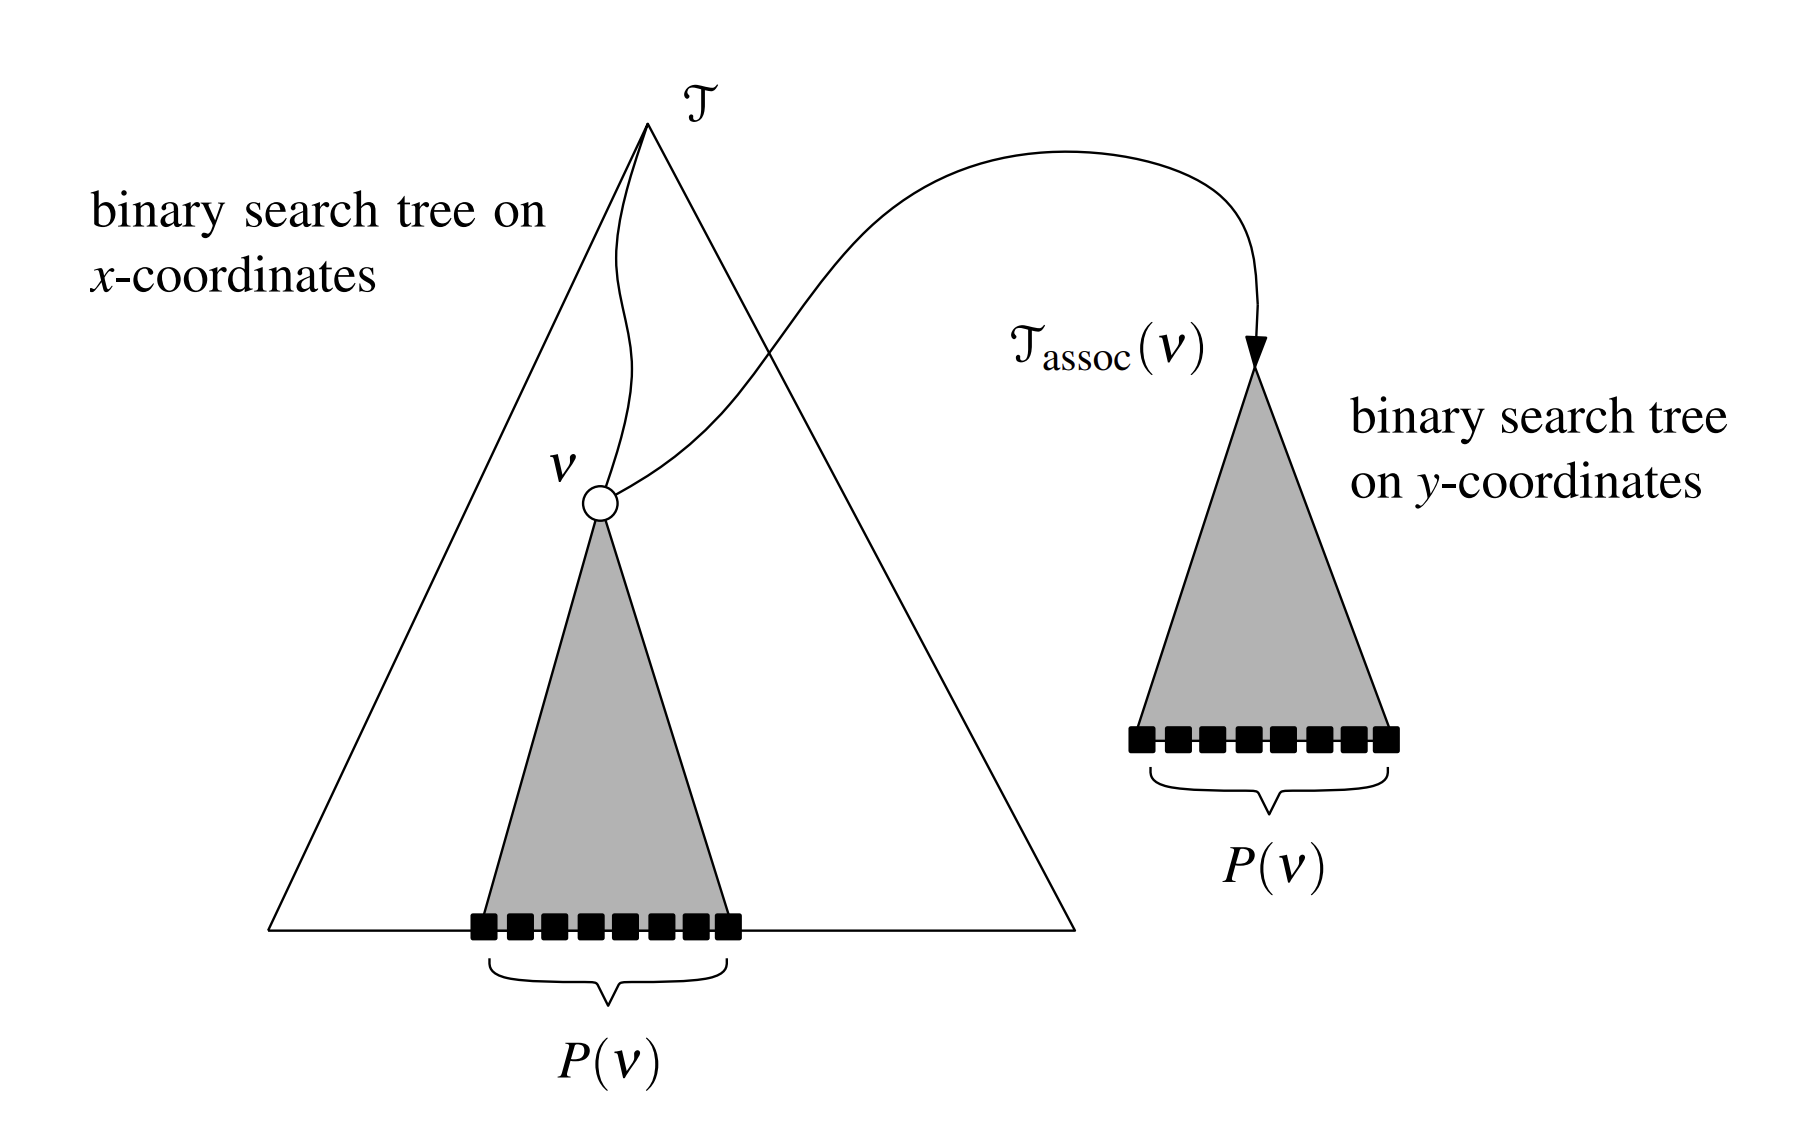
\includegraphics[width=0.7\textwidth]{treap-range-img/rangetree.png}
    \caption{2D Range-дерево}
    \label{rangetree}
\end{figure}

\textbf{Алгоритм построения} \textsc{Build2DRangeTree}$(P)$: рекурсивно строим главное дерево по $x$. В каждой вершине сначала строим $T_{\mathrm{assoc}}$ по $y$, после рекурсивно строим для точек с $x$ меньше медианы и больше медианы, после к точке с медианным $x$ слева и справа подвешиваем результаты работы рекурсии, а ассоциированной структурой для нее назначим построенный ранее $T_{\mathrm{assoc}}$. При всем этом поддерживаем два отсортированных списка~--- по $x$ и по $y$ для $P(\nu)$ для всех $\nu$. Тогда $T_{\mathrm{assoc}}$ для $P$ строится за $O(|P|)$ (как в слиянии в mergesort).

\begin{lemma}
Range-дерево для $n$ точек плоскости использует $O(n \log n)$ памяти и строится за $O(n \log n)$.
\end{lemma}

\begin{proof}
Точка $p$ хранится ровно в одном $T_{\mathrm{assoc}}(\nu)$ для каждого уровня глубины. Уровней $O(\log n)$, на каждом суммарно $O(n)$ точек, значит суммарная память $O(n \log n)$. Каждый лист на любой глубине участвует в $O(1)$ операциях, значит аналогично время работы $O(n \log n)$ (еще сортировка по $x$ в самом начале, но она не влияет на временную сложность).
\end{proof}

\subsection{Алгоритм запроса}
Сначала выбираем точки с $x$-координатой в $[x:x']$ как в \textsc{1DRangeQuery} (но пока ничего не возвращаем)~--- это $O(\log n)$ канонических подмножеств из BST по $x$. Затем в каждом из них ищем точки с $y$-координатой в $[y:y']$ с помощью вспомогательных BST по $y$, здесь уже просто стандартный \textsc{1DRangeQuery}.

\begin{lemma}
Запрос к двумерному range-дереву из $n$ точек работает за $O(\log^2 n + k)$.
\end{lemma}

\begin{proof}
Главное дерево посещает $O(\log n)$ вершин на каждом из двух путей поиска. В каждой из $O(\log n)$ выбранных вершин $\nu$ выполняется \textsc{1DRangeQuery} за $O(\log n + k_\nu)$. Суммарно: $\sum_\nu O(\log n + k_\nu) = O(\log^2 n) + O(k)$.
\end{proof}

\begin{theorem}
Range-дерево для $n$ точек плоскости использует $O(n\log n)$ памяти, строится за $O(n\log n)$, ответ на запрос тратит $O(\log^2 n + k)$ времени.
\end{theorem}

\begin{remark}
    Время на ответ на запрос мы скоро улучшим.
\end{remark}

\subsection{Многомерные range-деревья}

Обобщение на $d$ измерений строится рекурсивно: главное дерево~--- BST по первой координате; ассоциированная структура каждой вершины~--- $(d-1)$-мерное range-дерево по оставшимся $d-1$ координатам. Рекурсия заканчивается при $d=2$.

Запрос делается аналогично: в главном дереве выбираем $O(\log n)$ канонических подмножеств, в каждом из них делаем $(d-1)$-мерный запрос. На $i$-м уровне рекурсии имеется $O(\log^i n)$ канонических подмножеств.

\begin{theorem}
$d$-мерное range-дерево для $n$ точек использует $O(n\log^{d-1} n)$ памяти, строится за $O(n\log^{d-1} n)$, запросы отвечаются за $O(\log^d n + k)$.
\end{theorem}

\begin{proof}
Обозначим $T_d(n)$ ~--- время построения для $d$ измерений и $Q_d(n)$~--- время запроса для $d$ измерений (без учёта возврата точек, то есть только на нахождение канонических подмножеств по всем размерностям).

\textit{Построение:} $T_d(n) = O(n\log n) + O(\log n) \cdot T_{d-1}(n)$, первое слагаемое из построения BST, а второе поскольку на каждом из $O(\log n)$ уровней главного дерева точка входит ровно в одну ассоциированную структуру. С учётом $T_2(n) = O(n\log n)$ по индукции $T_d(n) = O(n\log^{d-1} n)$. Память аналогично.

\textit{Запрос:} $Q_d(n) = O(\log n) + O(\log n) \cdot Q_{d-1}(n)$. Первое слагаемое из поиска по дереву по первой координате, второе ~--- $O(\log n)$ вызовов запроса меньшей размерности. $Q_2(n) = O(\log^2 n)$ по индукции $Q_d(n) = O(\log^d n)$. Осталось прибавить $O(k)$ на возвращение значений точек.
\end{proof}


\subsection{Fractional Cascading и Layered Range-Tree}
Улучшим время на запрос для плоскости до $O(\log n + k)$, назовем эту структуру \textit{2D layered range-tree}, и используем ее для рекурсивного построения, как в range-tree. Из анализа времени на запрос для range-tree видно, что в $\mathbb{R}^d$ время на запрос улучшится до $O(\log^{d - 1} n + k)$.

Сначала обсудим \textbf{fractional-cascading}. Эта техника опирается на следующее соображение. Пусть у нас есть два отсортированных массива чисел $A_1$ и $A_2$, причем $A_2$ является подмножеством $A_1$. Мы хотим ответить на обычный 1D запрос $[x:x']$. Можно было бы для каждого из массивов вызвать бинарный поиск для $x$, а после обойти все числа правее и вернуть их, пока они меньше $x'$, поэтому мы потратим $O(\log |A_1| + \log|A_2|+ k_1 + k_2)$ времени. Но мы хотим воспользоваться знанием $A_1 \supset A_2$! Давайте делать не так: для каждого элемента $\mu$ в $A_1$ будем хранить ссылку на первый элемент $A_2$, не меньший $\mu$. Теперь вызовем двоичный поиск для нижней границы в $A_1$, начнем идти вправо от найденного числа $t$, пока не встретим в $A$ первый элемент $>x'$. Аналогично можно сделать и для $A_2$, но в этот раз мы находим первый элемент $\geq x$ бесплатно ~--- просто берем ссылку, соответствующую $t$, после чего идти направо, пока не дойдем до числа $> x'$. Таким образом, для поиска в $A_1$ мы потратили $O(\log |A_1| + k_1)$, а в $A_2$ ~--- $O(1+k_2)$.

\begin{figure}[h!]
    \centering
    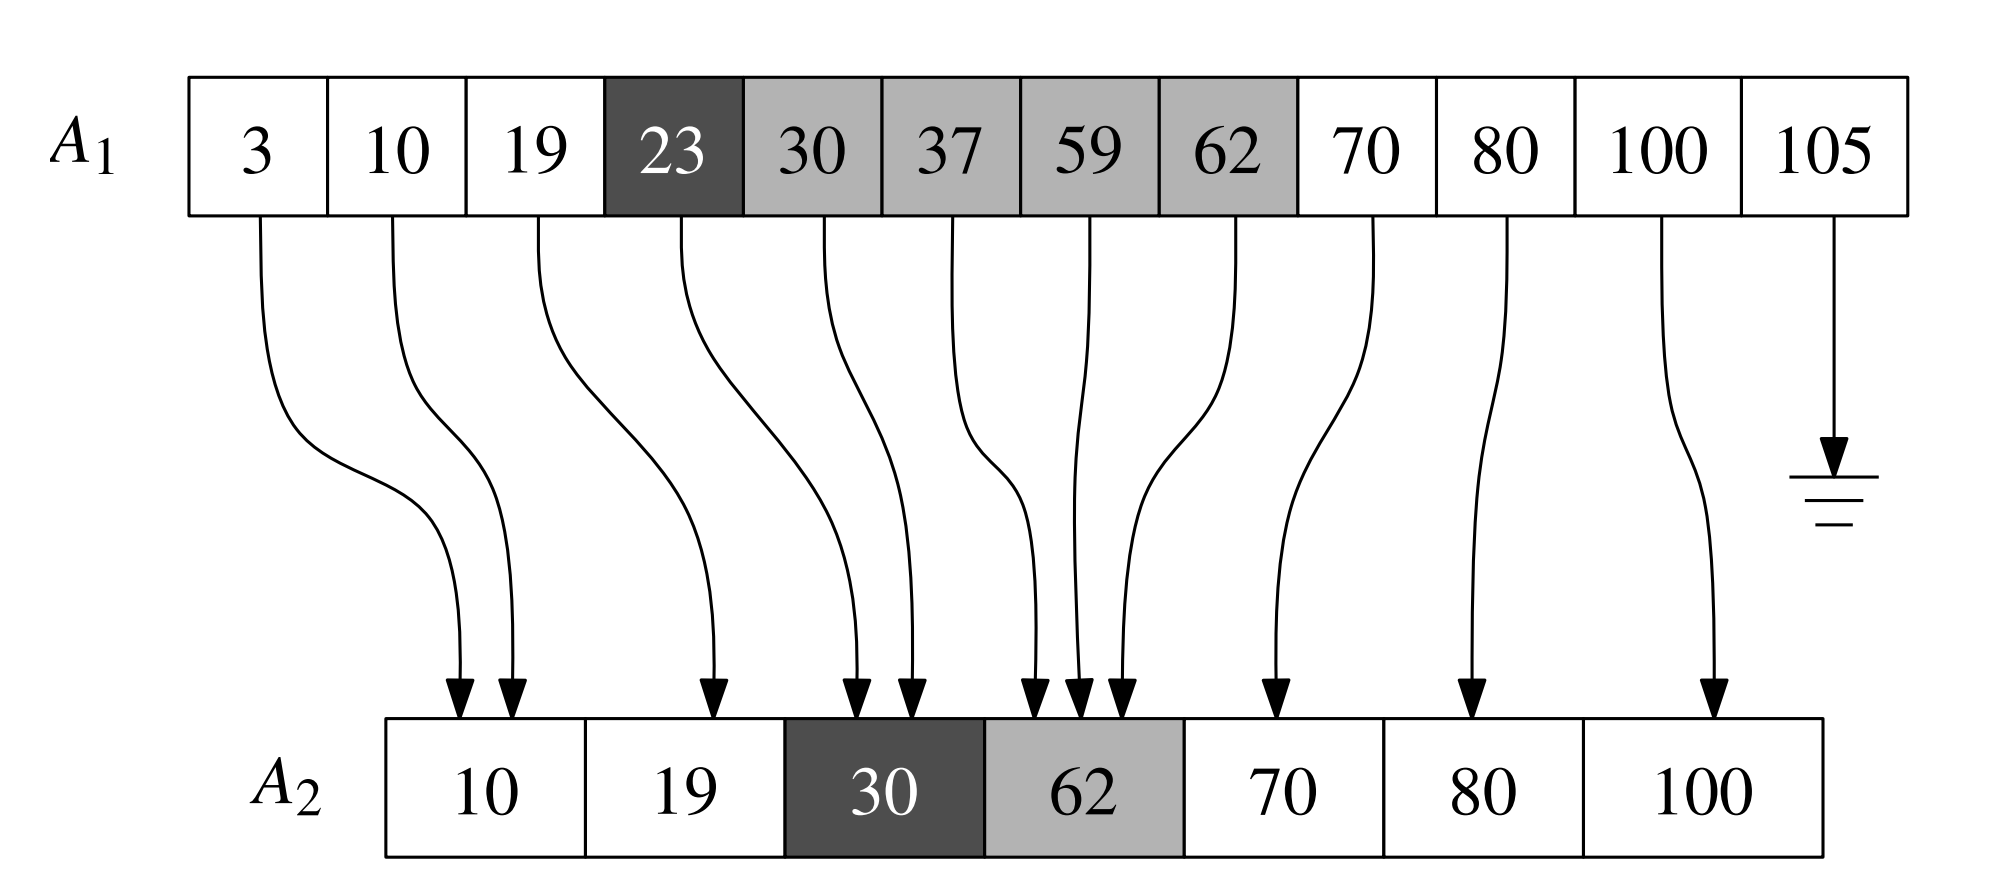
\includegraphics[width=0.7\textwidth]{treap-range-img/2arrays.png}
    \caption{Делаем запрос [20:65] для массивов $A_1$ и $A_2$}
    \label{2arrays}
\end{figure}

Теперь о применимости этой идеи к range-деревьям. Напомню, сейчас рассматриваем 2D реализацию. Заметим, что $P(\nu) = P(lc(\nu)) \bigsqcup P(rc(\nu))$ ($lc, rc$ - левый и правый ребенок). Тогда давайте заменим каждый BST $T_{\mathrm{assoc}}(\nu)$ на отсортированный массив $A(\nu)$. В каждой ячейке $A(\nu)[i]$ помимо точки храним два указателя~--- на ячейки $A(\mathrm{lc}(\nu))$ и $A(\mathrm{rc}(\nu))$, хранящие точку с наименьшей $y$-координатой $\geq$ текущей (прямо как в fractional-cascading). Такую модифицированную версию range-tree называют \textbf{Layered range-tree}.

\textbf{Как работает запрос.} Как и раньше, мы ищем те $O(\log n)$ вершин, чьи канонические подмножества представляют интересующий отрезок по $x$ координате, но теперь мы делаем один двоичный поиск по $y$. В $\nu_{\mathrm{split}}$ делаем двоичный поиск по $y$ за $O(\log n)$. Далее, спускаясь по главному дереву как в \textsc{1DRangeQuery}, поддерживаем первую позицию со значением $\geq y$ в массиве каждой посещённой вершины~--- она обновляется за $O(1)$ переходом по указателю. Для выбранной вершины $\nu$ сразу знаем стартовую позицию в $A(\nu)$, остаётся пройти вправо, пока $A(\nu)[i].y \leq y'$~--- это $O(1 + k_\nu)$. Просуммировав по $O(\log n)$ вершин, получим время $O(\log n + k)$.

В $d$ измерениях fractional-cascading убирает один множитель $\log n$, давая время запроса $O(\log^{d-1} n + k)$ при том же времени построения и памяти ($O(n\log^{d-1} n)$).

\begin{figure} \centering \vspace{-7mm}
  \input{treap-range-c/range-tikz}

  \caption{Множество точек в \(\mathbb{R}^2\) и запрос \([5, 12] \times [3, 9]\) (вверху, координаты «матричные»);
    2D range-дерево и переходы по ссылкам, соответствующие
    обработке этого запроса (внизу). Синим обведены вершины,
    накрывающие диапазон запроса по первой координате. Зелёная заливка~—
    точки, принадлежащие диапазону по второй координате.}
  \label{fig:range-tikz}
\end{figure}

\subsection{Совпадающие координаты}

До сих пор предполагалось, что все $x$ и $y$ координаты различны. Это ограничение снимается переходом в \textit{composite-number space}.

Для построения дерева по сути только требовалось, чтобы мы могли сравнивать числа в нем. Каждую точку $p = (p_x, p_y)$ заменяем на $\hat{p} = ((p_x | p_y),\, (p_y | p_x))$, где $(a | b)$~--- пара вещественных чисел с лексикографическим порядком: $(a|b) < (a'|b') \Leftrightarrow a < a'$ или $(a = a'$ и $b < b')$. При такой замене и первые, и вторые координаты всех точек попарно различны, что и нужно для построения дерева.

Запрос $[x:x'] \times [y:y']$ преобразуется в $[(x|-\infty):(x'|+\infty)] \times [(y|-\infty):(y'|+\infty)]$.

\end{document}